\documentclass[final]{beamer}

% Packages
\usepackage[scale=1.24]{beamerposter}
\usepackage{graphicx}
\usepackage{booktabs}
\usepackage{amssymb}
\usepackage{amsmath}
%\usepackage{minted}
\usepackage{listings}
\usepackage{xcolor}
\usepackage{tikz}

\definecolor{darkgreen}{rgb}{0,0.6,0}
\lstdefinestyle{Python}{
    language        = Python,
    basicstyle      = \ttfamily,
    keywordstyle    = \color{blue},
    keywordstyle    = [2] \color{teal}, % just to check that it works
    stringstyle     = \color{green},
    commentstyle    = \color{darkgreen}\ttfamily
}

% Styling
\newcommand{\agsNote}[1]{\textcolor{cyan}{#1}}
\newcommand{\bfCenter}[1]{\centerline{\textbf{#1}}}
\usetheme{confposter}
\setbeamercolor{block title}{fg=blue,bg=white}
\setbeamercolor{title}{fg=red,bg=white}
\setbeamercolor{block body}{fg=black,bg=white}
\setbeamercolor{block alerted title}{fg=white,bg=blue}
\setbeamercolor{block alerted body}{fg=black,bg=white}

% Formatting
\newlength{\sepwid}
\newlength{\onecolwid}
\newlength{\twocolwid}
\newlength{\threecolwid}
\setlength{\paperwidth}{48in}
\setlength{\paperheight}{36in}
\setlength{\sepwid}{0.024\paperwidth}
\setlength{\onecolwid}{0.2\paperwidth}
\setlength{\twocolwid}{0.464\paperwidth}
\setlength{\threecolwid}{0.706\paperwidth}
\setlength{\topmargin}{-1.6in}

\newcommand{\dif}{\mathrm{d}}
\newcommand{\bvec}[1]{\boldsymbol{#1}}
\newcommand{\vx}{\bvec{x}}
\newcommand{\vt}{\bvec{t}}

% Meta Data
\title{Community Supported Quasi-Monte Carlo (QMC) Software}
\author{ Aleksei Sorokin (\texttt{asorokin@hawk.iit.edu}), Sou-Cheng Choi (\texttt{schoi32@iit.edu}), Fred Hickernell (\texttt{hickernell@iit.edu}) }
\institute{Department of Applied Mathematics, Illinois Institute of Technology\vspace{-2ex}}

 
\begin{document}
% logos
\addtobeamertemplate{headline}{} 
{
	\begin{tikzpicture}[remember picture,overlay] 
	\node [anchor=north west, inner sep=1.5cm] at (current page.north west) {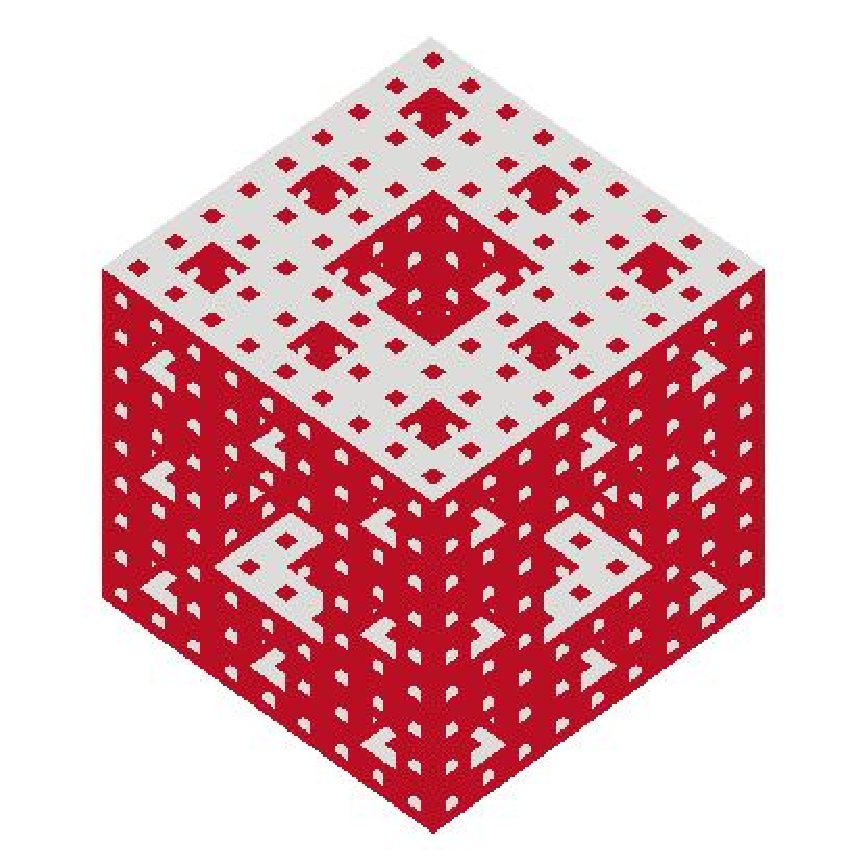
\includegraphics[height=8cm]{images/MengerIITRedGray.eps}}; 
	\end{tikzpicture} 
}

\addtobeamertemplate{headline}{} 
{
	\begin{tikzpicture}[remember picture,overlay] 
	\node [anchor=north east, inner sep=1.5cm] at (current page.north east) {
\includegraphics[height=8cm]{images/iit_high_res.png}}; 
	\end{tikzpicture} 
}

% Setup Format and Styling
\addtobeamertemplate{block end}{}{\vspace*{2ex}}
\addtobeamertemplate{block alerted end}{}{\vspace*{2ex}}
\setlength{\belowcaptionskip}{2ex}
\setlength\belowdisplayshortskip{2ex}
\begin{frame}[t]
\vspace{-2ex}
\begin{columns}[t]

% Column 1
\begin{column}{\sepwid}\end{column}
\begin{column}{\threecolwid}
\begin{columns}[t,totalwidth=\threecolwid]  

\begin{column}{\onecolwid}\vspace{-1in}
%~~~~~~~~~~~~~~~~~~~~~~~~~~~~~~~~~~~~~~~~~~~~~~~
%    Software Objectives
%~~~~~~~~~~~~~~~~~~~~~~~~~~~~~~~~~~~~~~~~~~~~~~~
\begin{block}{Software Objectives}
    To provide QMC software \cite{HicEtal19} that is: 
    \begin{itemize}
        \item comprised of free open source tools
        \item designed for continuous development
        \item easy to use for non-experts
        \item a recognized standard
    \end{itemize}
\end{block}

%~~~~~~~~~~~~~~~~~~~~~~~~~~~~~~~~~~~~~~~~~~~~~~~
%    The QMC Problem
%~~~~~~~~~~~~~~~~~~~~~~~~~~~~~~~~~~~~~~~~~~~~~~~
\vspace{-2ex}
\begin{block}{The Integration Problem}
    \bfCenter{Original Form}
        \begin{equation*}
            \mu = \int_{T} g(t) \, \lambda(\dif t) 
            \label{eq:ogProblem}
        \end{equation*}
        $ g:T \rightarrow \mathbb{R}  $ is original integrand \\
        $ \lambda $ is original measure

    \vspace{2ex}
    \bfCenter{Convenient Form}
        \begin{equation*}
            \mu = \int_{X} f(x)\rho(x)\, dx = \int_{X} f(x) \, \nu( \dif x)
            \label{convForm}
        \end{equation*}
	$f: X \rightarrow \mathbb{R} $ is integrand after change of variables\\
        $\nu  $ is some well defined probability measure\\
        $\rho: X \rightarrow T $ is the probability density
       
        
    \vspace{2ex}
    \bfCenter{(Quasi-)Monte Carlo Approximation}
        \begin{gather*}
            \hat{\mu}_n = a_n \sum_{i=1}^{n} f(x_i)w_i =  \int_{X} f(x) \, \hat{\nu}( \dif x)
            \label{qmcApprox}
	\\ \nu  \approx \hat{\nu}_n = a_n \sum_{i=1}^n w_i \delta_{x_i}(\cdot) 
            \text{ is discrete probability measure}
        \end{gather*}
\end{block}
\end{column}


%~~~~~~~~~~~~~~~~~~~~~~~~~~~~~~~~~~~~~~~~~~~~~~~
%   Building blocks
%~~~~~~~~~~~~~~~~~~~~~~~~~~~~~~~~~~~~~~~~~~~~~~~
\begin{column}{\twocolwid}\vspace{-1in}
\begin{block}{Main Object Classes}
%--------------------------------------------------------------
The routine \texttt{integrate} accepts instances of concrete subclasses of four abstract  classes that  represent the integrand,
original measure, discrete distribution associated with the sampling points, and stopping criterion.
%    Integrate
\begin{column}{\onecolwid}  \vspace{-2ex}
\setbeamercolor{block alerted title}{fg=black,bg=red!10}
\begin{alertblock}{\texttt{integrate}}
    Given $\epsilon>0$, find $\hat{\mu}_n$ such that $\left | \mu - \hat{\mu}_n \right  | \leq \epsilon$ \\[1ex]~\
    \textbf{Arguments}
    \begin{itemize}
        \item Function instance
        \item Measure instance
        \item Discrete Distribution instance
        \item Stopping Criteria instance
    \end{itemize}
\end{alertblock}

%    Function
\vspace{-.1in}
\setbeamercolor{block alerted title}{fg=black,bg=green!10}
\begin{alertblock}{Function}
    Specify and generate values $f(x_i)$ \\[1ex]~\
    \textbf{Concrete Classes}
    \begin{itemize}
        \item Keister functions \cite{keister1996multidimensional}
        \item Asian call option's payoff 
    \end{itemize}
\end{alertblock}

%    Discrete Distribution
\vspace{-.1in}
\begin{alertblock}{Discrete Distribution, $\hat{\nu}$}
    Specify and generate $a_n \sum_{i=1}^n w_i \delta_{x_i}(\cdot)$ \\[1ex]~\
    \textbf{Concrete Classes}
    \begin{itemize}
        \item IID
        \item QMC (Lattice \& Sobol) \cite{kuo2016application,nuyensmagic}
    \end{itemize}
\end{alertblock}
\end{column} 
%--------------------------------------------------------------
%--------------------------------------------------------------
%    Stopping Criterion
\begin{column}{\onecolwid}   \vspace{-2ex}
\setbeamercolor{block alerted title}{fg=black,bg=green!10}
\begin{alertblock}{Stopping Criterion}
    Determine sample size, $n$, given $\epsilon$\\[1ex]~\
    \textbf{Concrete Classes}
    \begin{itemize}
        \item Central limit theorem (IID)
        \item Mean Variance (Mesh)
    \end{itemize}
\end{alertblock}

%    Measure
\vspace{.4in}
\begin{alertblock}{Measure, $\lambda$ and $\nu$}
    Specify the original measure and convienient probability measure \\[1ex]~\
    \textbf{Implemented Functions}
    \begin{itemize}
        \item Standard uniform
        \item Standard Gaussian
        \item IID zero-mean Gaussian
        \item Brownian motion 
    \end{itemize}
\end{alertblock}

%    Accumulate Data
\vspace{.4in}
\begin{alertblock}{Accumulate Data}
    Accumulate data required for the computation of the integral and the stopping criterion
\end{alertblock}
\end{column}

%--------------------------------------------------------------
\end{block}
\end{column}

\end{columns} 

%%%%%%%%%%%%%%%%%%%%%%%%%%%%%%%%%%%%
% Python Examples
%%%%%%%%%%%%%%%%%%%%%%%%%%%%%%%%%%%%
\begin{column}{\threecolwid}\vspace{-0.8in}
\begin{block}{Python Examples}
    \begin{column}{\onecolwid}
	\vspace{.5in}
        %\inputminted{python}{Keister.snip.py}
        \lstinputlisting[style=Python,caption=Essential code for estimating the Keister integral in the first subplot of Figure~1.]{Keister.snip.py}
    \end{column}
	\begin{column}{\twocolwid}
     % \vspace{-2ex}
        \begin{figure} 
            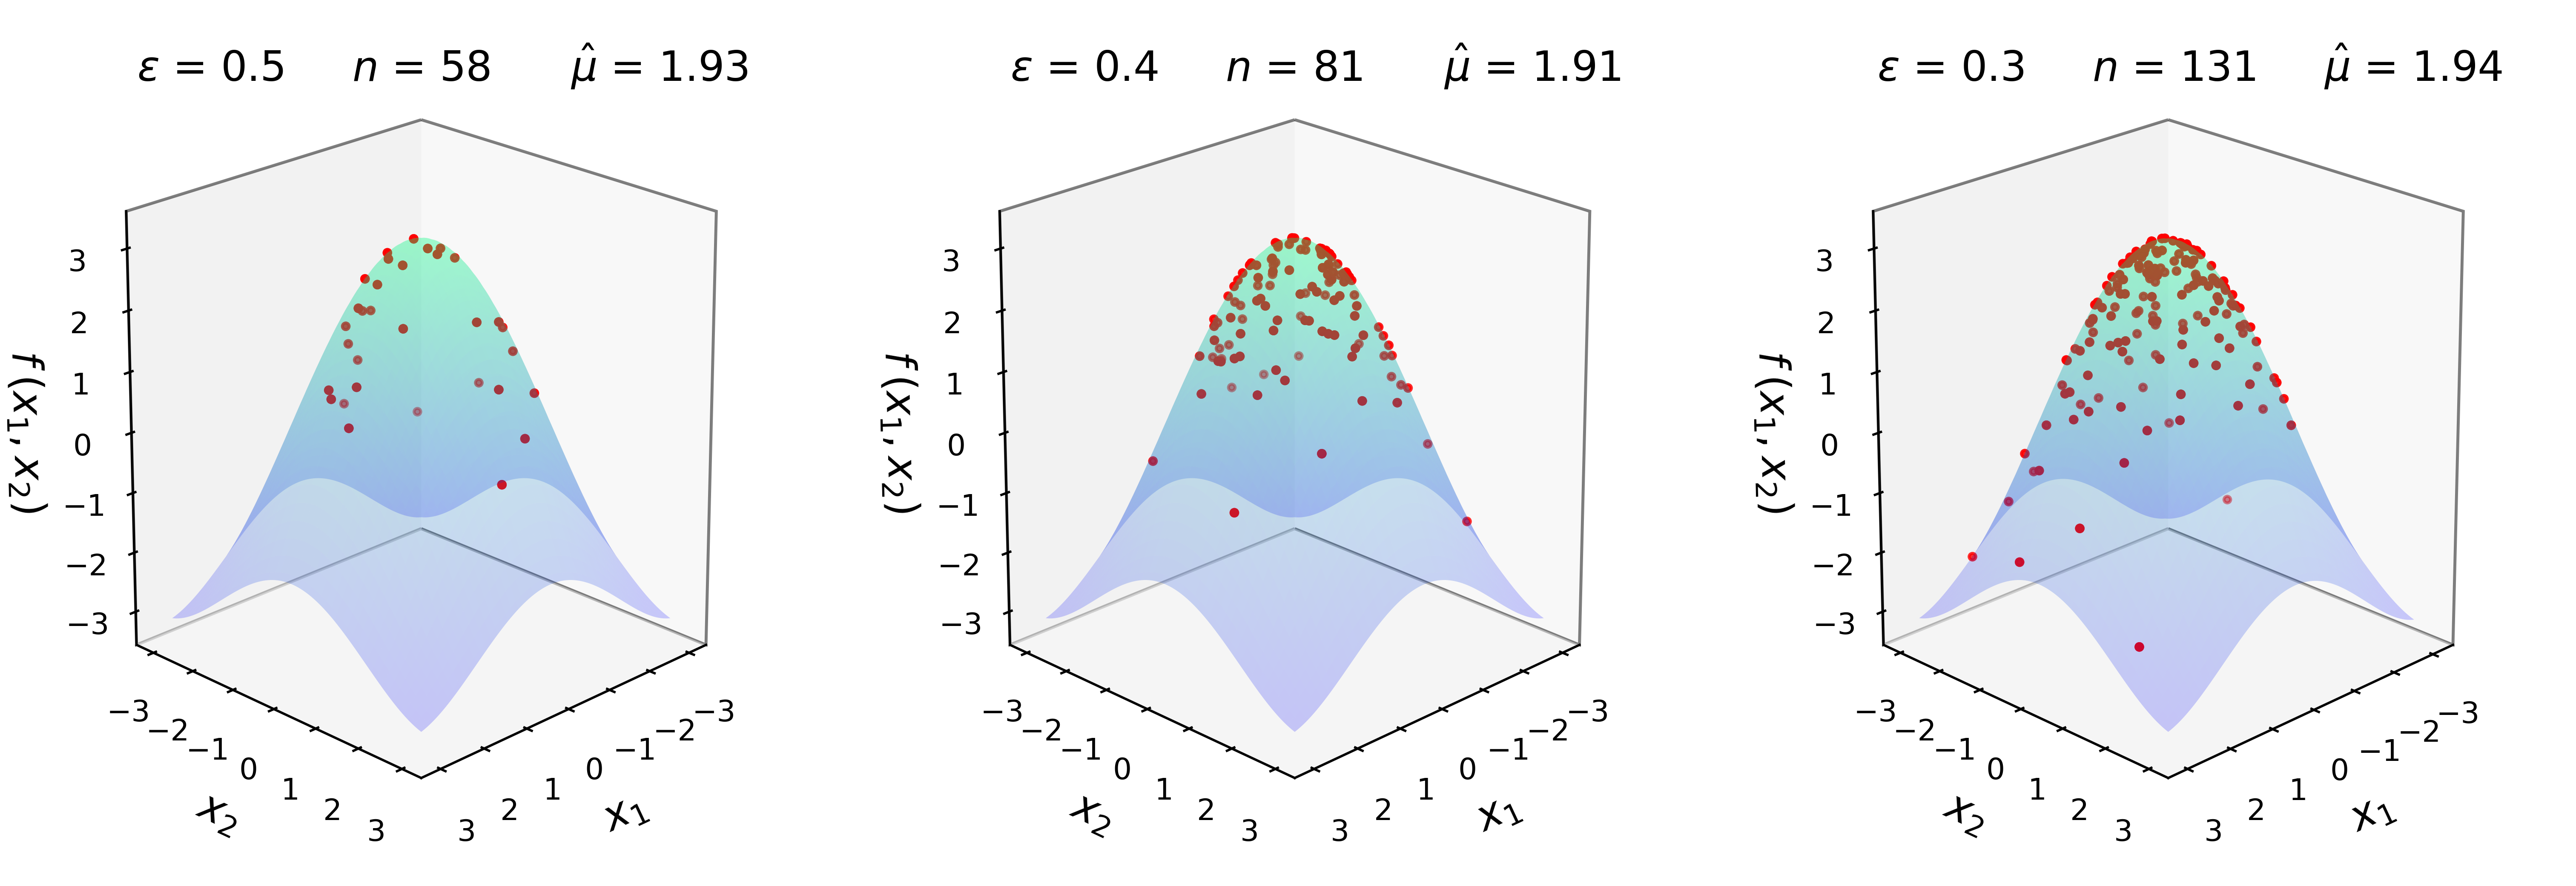
\includegraphics[width=0.96\textwidth]{Images/Three_3d_SurfaceScatters.png}         
            \caption{\ Reducing tolerance automatically results in more samples and better approximations of the Keister integral~\cite{keister1996multidimensional},  
$\displaystyle \int_{\mathbb{R}^d} \pi^{d/2} \cos(\lVert \vt \rVert) \, \frac{\exp(-\lVert \vt \rVert^2)}{\pi^{d/2}}\,\dif \vt = 
 \int_{\mathbb{R}^d} \pi^{d/2} \cos(\lVert \vx \rVert /\sqrt{2}) \, \frac{\exp(-\lVert \vx \rVert^2/2)}{(2\pi)^{d/2}}\,\dif \vx
%\int_{[0,1]^d} \pi^{d/2} \cos\left(\sqrt{ \frac 12 \sum_{j=1}^d[\Phi^{-1}(x_j)]^2}\right)  \, \dif \vx 
\approx 1.80819 $  with $d=2$ and where $\Phi$ is the  standard normal  cumulative distribution function. This figure is reproducible by \texttt{Test\_3D\_Point\_Distribution.py}~\cite{HicEtal19}.}  \label{fig3d}
        \end{figure} 
    \end{column}

\end{block}
\end{column}

\end{column}

%----------------------------------------------------------------------------------------
% Results
%----------------------------------------------------------------------------------------
\begin{column}{\sepwid}\end{column}
\begin{column}{\onecolwid}\vspace{-.3in}
\begin{block}{Results}
    \bfCenter{Integration Time Comparison}
    \vspace{-.7in}
    \begin{figure}
        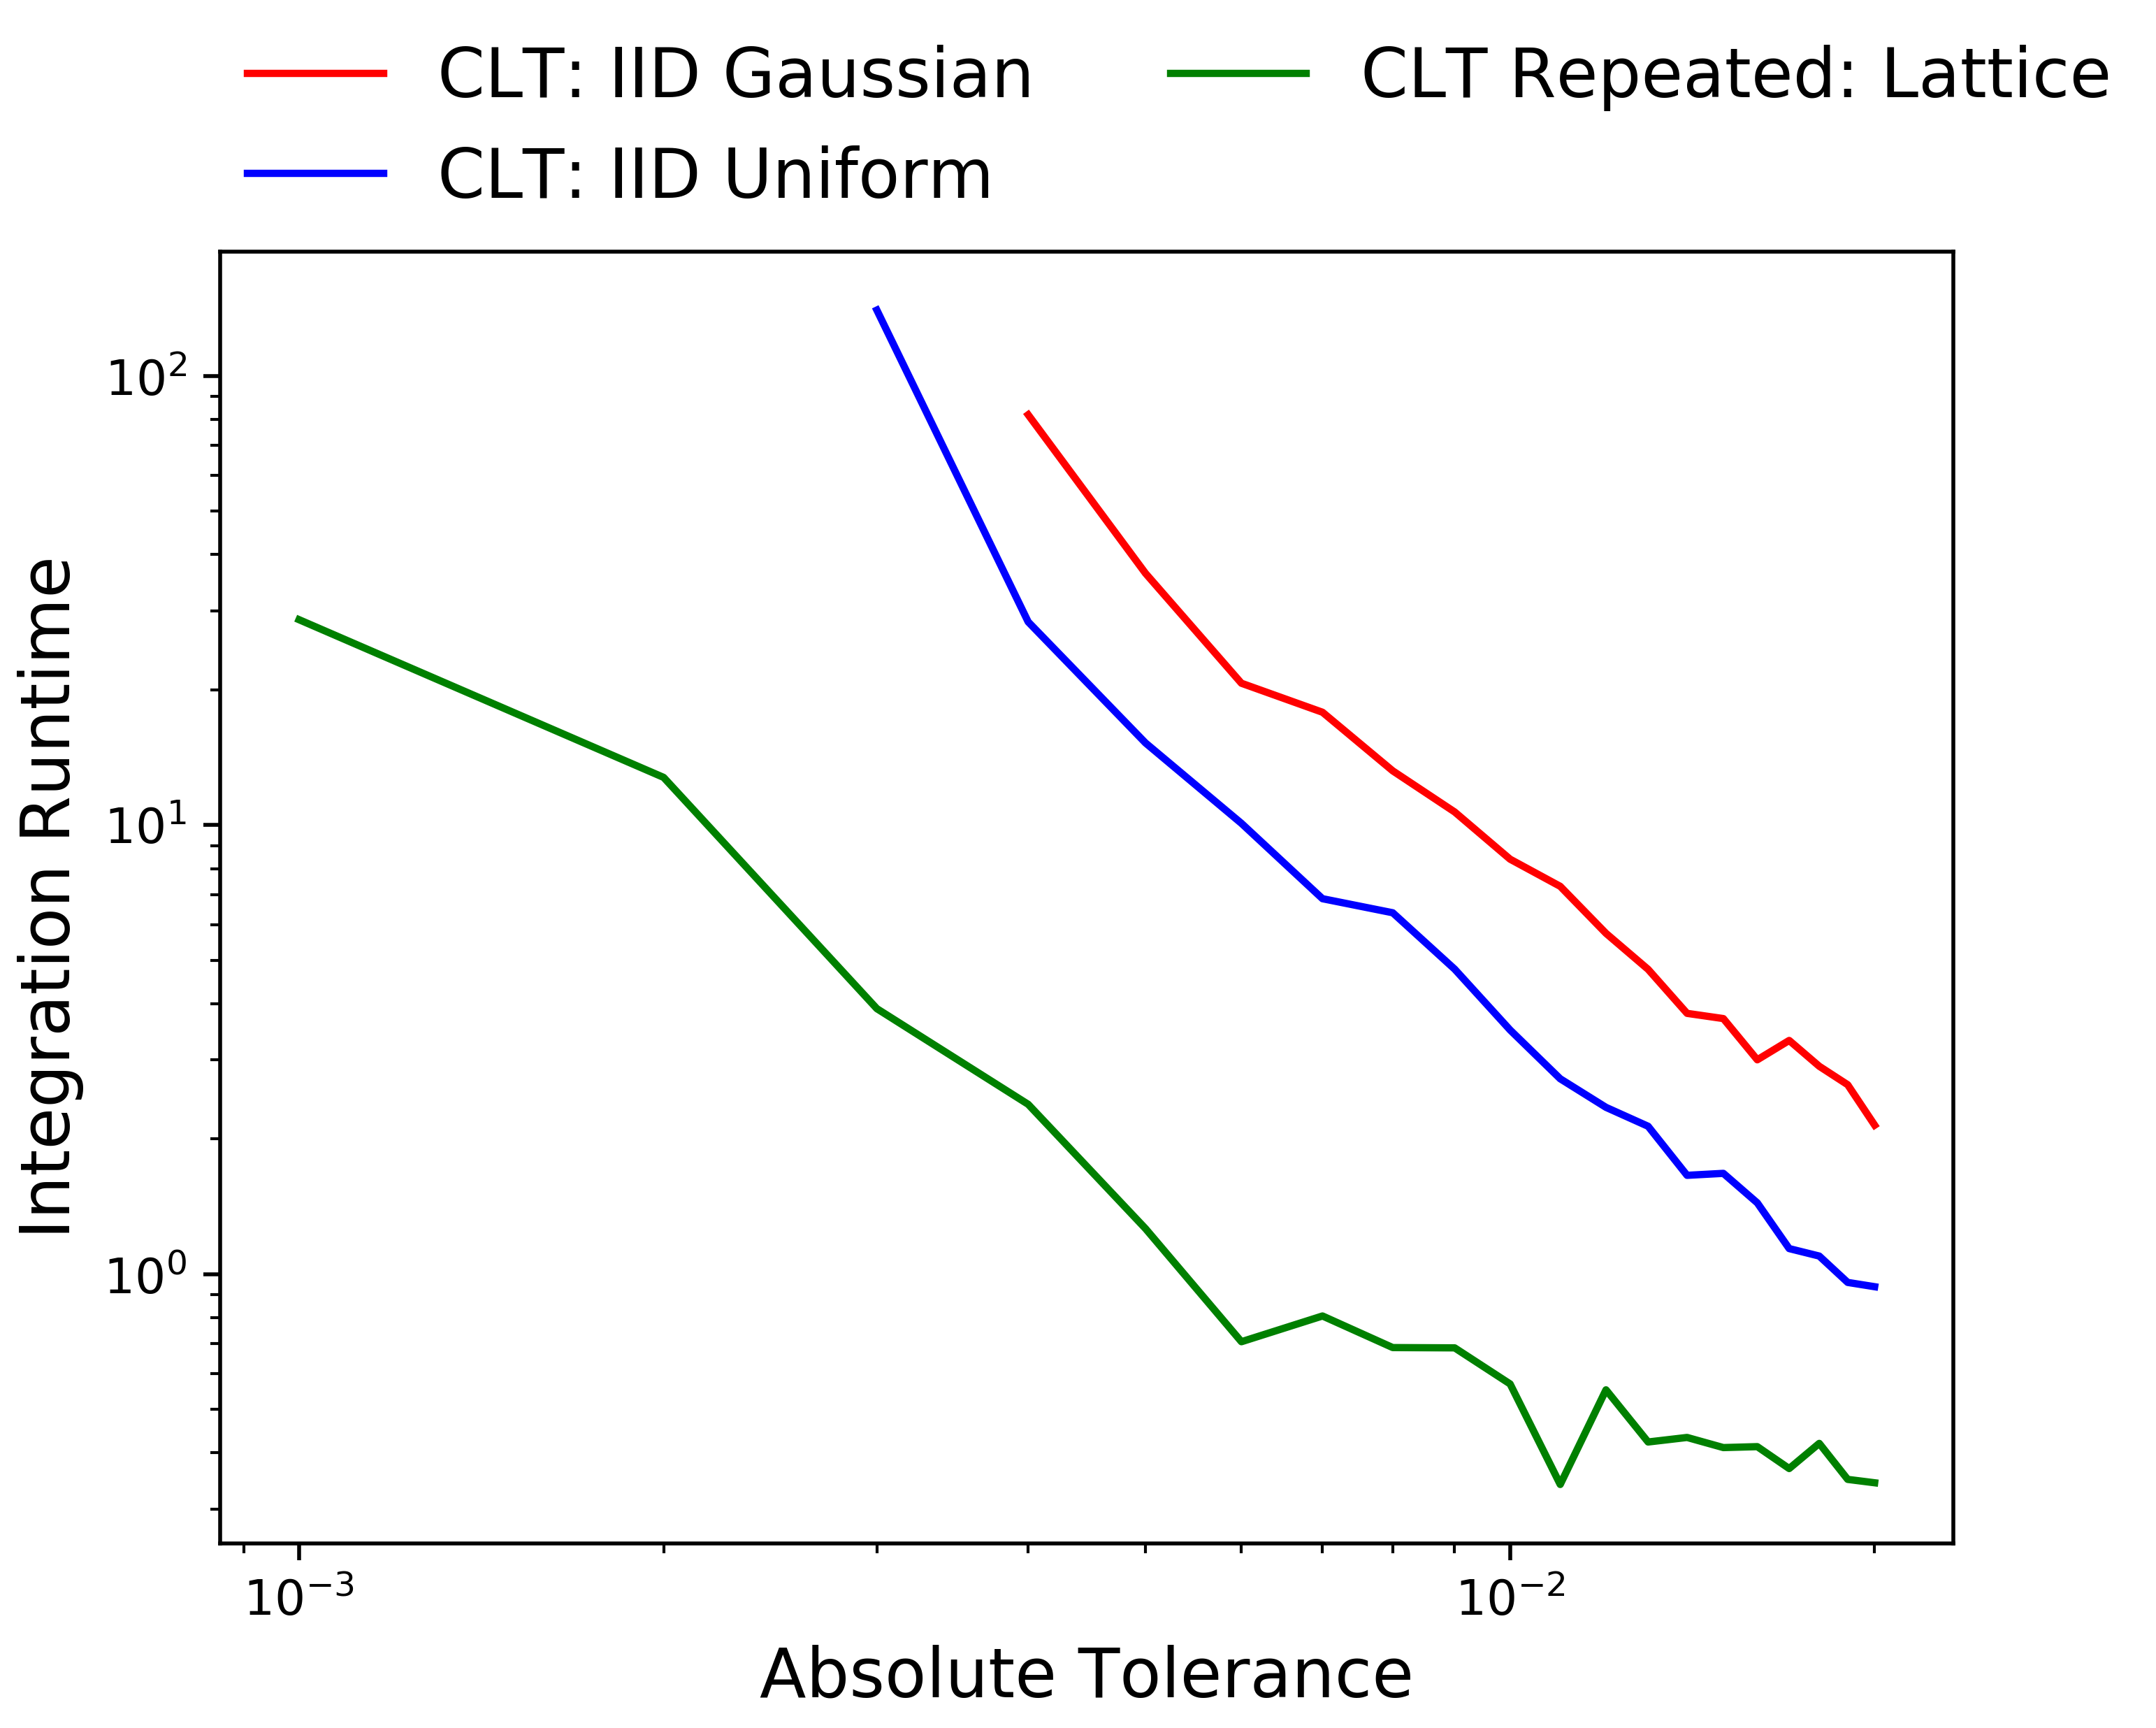
\includegraphics[width=1.05\textwidth]{Images/AbsTol_Runtime_LinePlot.png}
        \vspace{-1ex}
        \caption{\ Multi-dimensional Asian call option integrated with respect to Brownian Motion. This figure can be easily reproduced by \texttt{Test\_AbsTol\_RunTime.py}~\cite{HicEtal19}.}
    \end{figure}
\end{block}

%----------------------------------------------------------------------------------------
%    Future Work
%---------------------------------------------------------------------------------------- 
\vspace{-.9in}
\begin{block}{Future Work}
    \begin{itemize}
        \item Enhance tests, examples, and documentation
        \item Refine existing code. e.g. improve Sobol speed
        \item Bring in relevant algorithms from GAIL~\cite{ChoEtal19}
        \item Expand community of contributors
    \end{itemize}
\end{block}

%----------------------------------------------------------------------------------------
%	REFERENCES
%----------------------------------------------------------------------------------------
\vspace{-.5in}
\begin{block}{References}

\nocite{*} % Insert publications even if they are not cited in the poster
\small{\bibliographystyle{ieeetr}  %{abbrv}
\bibliography{main}}

\end{block}

%----------------------------------------------------------------------------------------
%	ACKNOWLEDGEMENTS
%----------------------------------------------------------------------------------------
%\vspace{-.3in}
%\begin{block}{Acknowledgements}
%    We thank Dirk Nuyens for providing the lattice and Sobol generators \cite{nuyensmagic}
%\end{block}
\end{column}
\end{columns}
\end{frame}
\end{document}
